\title{Process}

In this section, we will outline and explain how we transitioned from our initial phase and organized our project in order to facilitate work on practical implementation. We will explain which tools we utilized and the methodology we used to achieve our results.  \\

While the hermeneutic methodology facilitated invaluable insights during the exploratory stage of our project, its emphasis on interpretation and understanding proved less applicable when transitioning from knowledge acquisition to knowledge application. The hermeneutic approach, with its focus on understanding texts or phenomena in depth, provides a foundation for comprehensive understanding rather than prioritizing explicit task completion. Consequently, as the project shifted to a phase demanding direct action and the tangible execution of tasks, the inherent characteristics of the hermeneutic approach were less aligned with these new requirements. Therefore, to maintain project efficiency during the implementation phase, it became necessary to consider alternative methodologies more attuned to the objectives of this new stage.\\

We decided that our project demands were best met using an agile methodology. This methodology is an iterative approach to software development and project management that emphasizes flexibility, collaboration, and client satisfaction. It advocates adaptive planning, evolutionary development, early delivery, continual improvement, and encouraging rapid and flexible response to change. Agile methods break tasks into smaller increments with minimal planning and do not directly involve long-term planning. This methodology prioritizes direct communication over extensive documentation, producing working software that evolves through a collaborative effort between self-organizing cross-functional teams. \\

\begin{figure}[H]
    \centering
    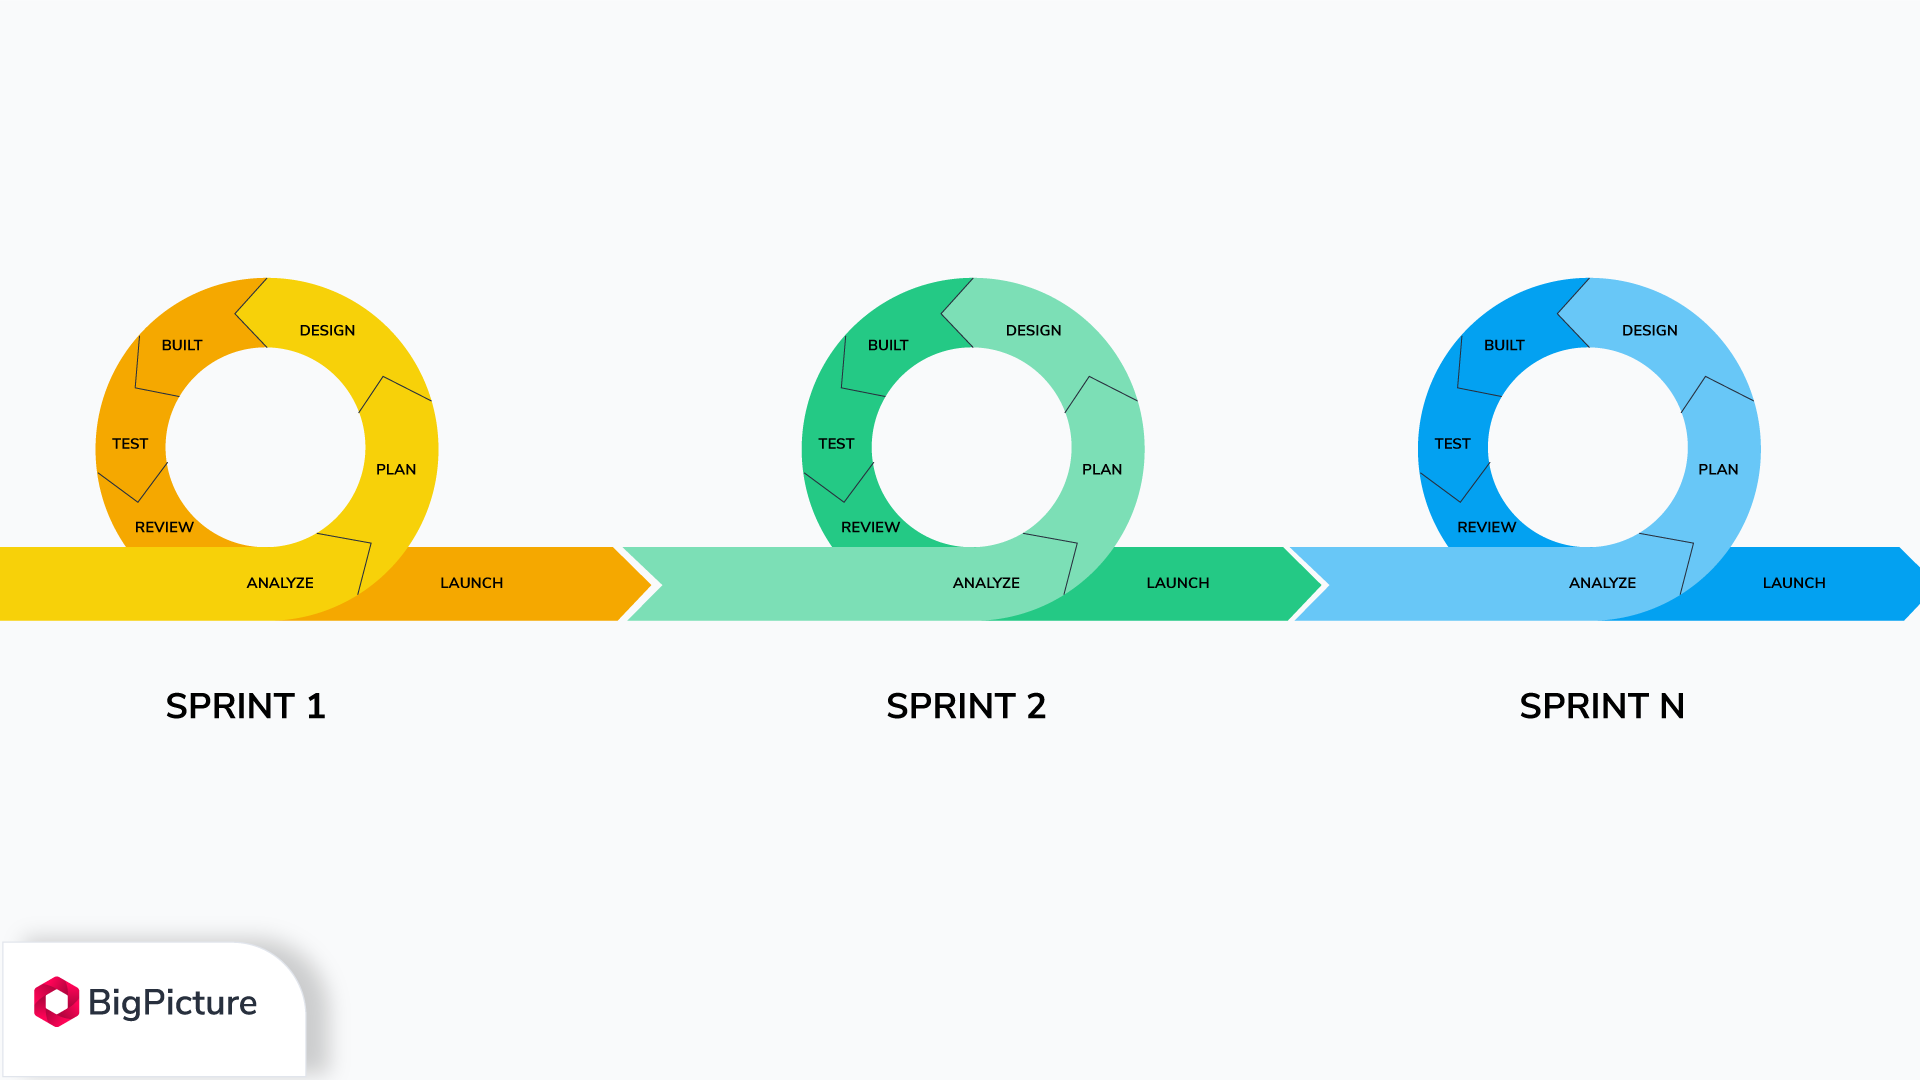
\includegraphics[scale=0.25]{fig/sprints.png}
    \caption{Sprint organization \cite{sprintimage}}
\end{figure}

An agile workflow has a number of key terms and features, and there are several different ways to conduct an agile project. Common for all of these, however, is that these projects are divided into short work cycles known as iterations or sprints, typically lasting between one and four weeks. Each sprint has a defined goal and a set of tasks to be completed. We decided that for our project we would not adhere to a strict definition, e.g., scrum. Instead, we opted to pick and choose between different features that made the most sense for our project, and to make sure that we utilized the most prominent features that are essential to an agile project. These features were: sprint, sprint backlog, daily stand-up meetings, and retrospective.\\

Following the agile methodology, we decided to have daily stand-up meetings where we would update the group on our individual progress. We organized our sprints to last one week at a time, where we had an initial meeting on Monday to set up our tasks for the week, and a meeting at the end of the week where we updated our client on where we were in terms of progress. In the end-of-week meetings, the client was invited to give feedback on which tasks they wanted us to prioritize going forward into the next sprint.\\

\section{Project Tools}

\subsection{Github}

We needed a way to organize and collaborate on code, and essential to this is Source Code Management (SCM), and for this purpose, our choice fell on git. Git is a distributed SCM, originally developed for use on the Linux kernel, but has since gained a significant market share and is now the dominant SCM. Git's primary function is to enable developers to create different versions of their projects and switch between these versions seamlessly. This means that developers can experiment with different features and code changes without impacting the main, stable codebase. If a change works well, it can be integrated (or "merged") into the main codebase; if not, it can be discarded without having caused any disruption.\\

In a team environment, Git is essential for managing contributions from multiple developers. Each developer can work on their own copy of the project (a "branch"), without interfering with others' work. When their work is complete, it can be merged into the main codebase.\\

Git is also distributed, meaning every developer has a complete copy of the project's history on their local machine. This not only allows developers to work offline but also provides an inherent backup. If any repository is lost, it can be restored from any developer's local copy.\\

Instead of organizing our own server with git, we opted for using GitHub, which allows students and educators access to their professional option at no cost, allowing us to organize our code in a more structured manner. \\

\subsection{Taiga}
In order to organize our agile workflow we elected to use Taiga. It is a web-based tool that allows us to track sprints, tasks within sprints, and assign aforementioned tasks to specific members of the group, and additionally allow members to follow updates on a specific task. In addition to this, Taiga has integration with GitHub, allowing us to modify tasks from GitHub whenever we commit code in our repository there.


\begin{figure}[h]
    \centering
    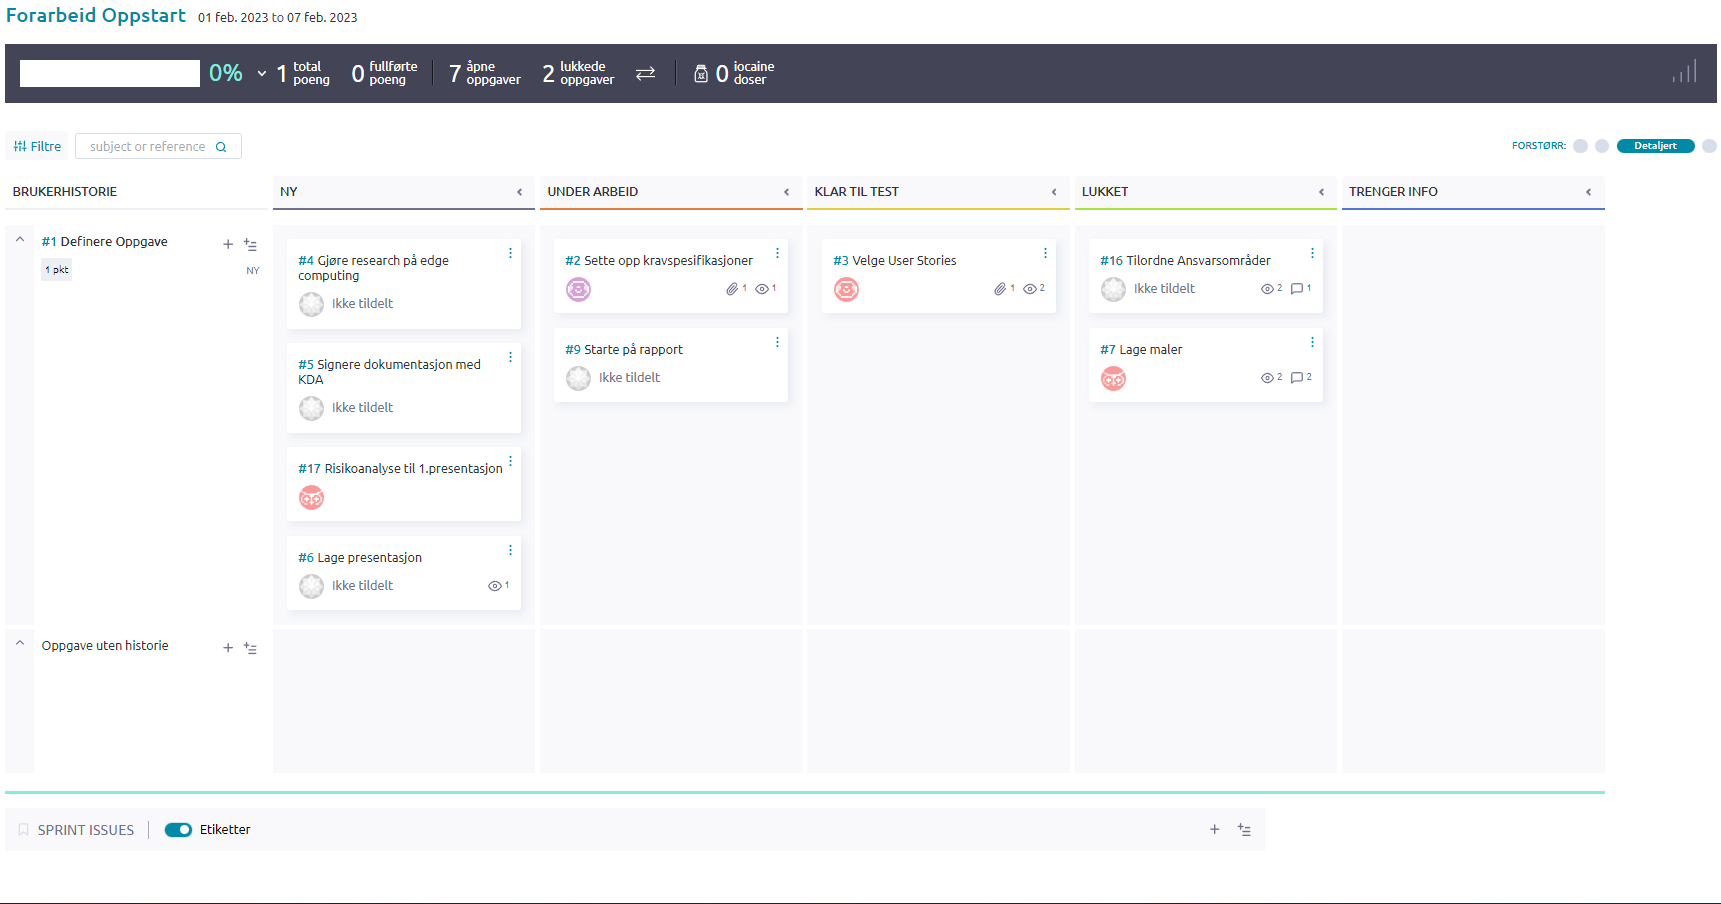
\includegraphics[width=\textwidth]{fig/Taiga eksempel.png}
    \caption{Taiga Interface}
\end{figure}

As the project progressed, we found that we were not generating a substantial amount of code, and therefore, the GitHub integration was not as crucial as we initially assumed. Moreover, our interaction with the Taiga platform was proving to be more of a diversion from our core tasks rather than a facilitator of our work. The platform's organization and functionality did not meet our needs and expectations, which caused further dissatisfaction. Consequently, we decided to transition away from this web-based project management tool. Instead, we opted for a more streamlined approach of crafting summaries for each sprint. This method proved to be less demanding in terms of resources and was more suitable and beneficial for the progression of our project.\\


\subsection{Overleaf}
Overleaf is a collaborative, cloud-based LaTeX editor used for the creation of scientific documents. LaTeX is a typesetting system favored in academia for its ability to handle technical and scientific documents with ease, especially those with complex mathematical equations or structures.\\

Overleaf provides a platform where multiple users can view, edit, and compile LaTeX documents in real time. This collaboration aspect makes it an excellent tool for group projects, theses, papers, or any document requiring input from several contributors.\\

\subsection{ChatGPT}
ChatGPT is an artificial intelligence language model, released to the public recently. It is designed to understand natural language and generate human-like responses to a wide range of prompts and questions.\\

ChatGPT is most useful for tasks that require natural language processing, such as language translation, sentiment analysis, text summarization, and conversational interfaces. It can also be used for a variety of other applications, such as content generation, language modeling, and knowledge extraction.\\

We have on occasion used ChatGPT for cleaning up and helping us formulate language in a more academic and formal fashion.\\

\subsection{Microsoft Suite}
Microsoft Office is a suite of productivity applications that have become a standard tool in most professional and academic environments. It includes software like Word for document creation, Excel for data management and analysis, PowerPoint for presentations, Outlook for email and calendar management, and more recently Teams for collaborative communication. Each of these applications serves distinct purposes and can be instrumental in managing and executing a project efficiently.\\

For our purposes, we organized a lot of our work through the university-provided teams solution, where we organized documents that were impractical to use LaTeX for. This is where we kept time sheets, presentation material, and meeting notes. \\

\newpage
\section{Risk Analysis}

Risk analysis is an ongoing process that continuously evaluates risk throughout the project's lifecycle. It is the responsibility of the risk manager to ensure that this process takes place regularly and consistently during the project. This is crucial because it raises awareness among us and our client about potential risks and vulnerabilities, encourages necessary improvements, and facilitates necessary changes. Such analysis can help the risk manager to identify new risks and changes that require attention along the way. \cite{Risk1}

After identifying the risks, it is essential to prioritize them based on their probability and consequence. Moreover, measures should be put in place to manage them effectively if they occur. While everyone on the team should participate in assessing the project's risks, the risk manager will be primarily responsible for ensuring quality assurance. \cite{Risk2}

\subsubsection{Identifying the risks in our project}
A risk analysis was conducted for our project, wherein we identified both internal and external risks. Internal risks are linked with factors that are under our control, whereas external risks are associated with factors that lie beyond our control.\cite{RiskInternalExternal}

After identifying the risks at this stage, we evaluate their potential consequences and determine the appropriate measures that can be taken if they occur. To gain a better overview, we record the risks in a table that includes a unique code, a description of the risk event, recommended measures, probability (P), consequence (C), and priority. Below is a comprehensive overview of both internal and external risks:


\begin{figure}
\centering
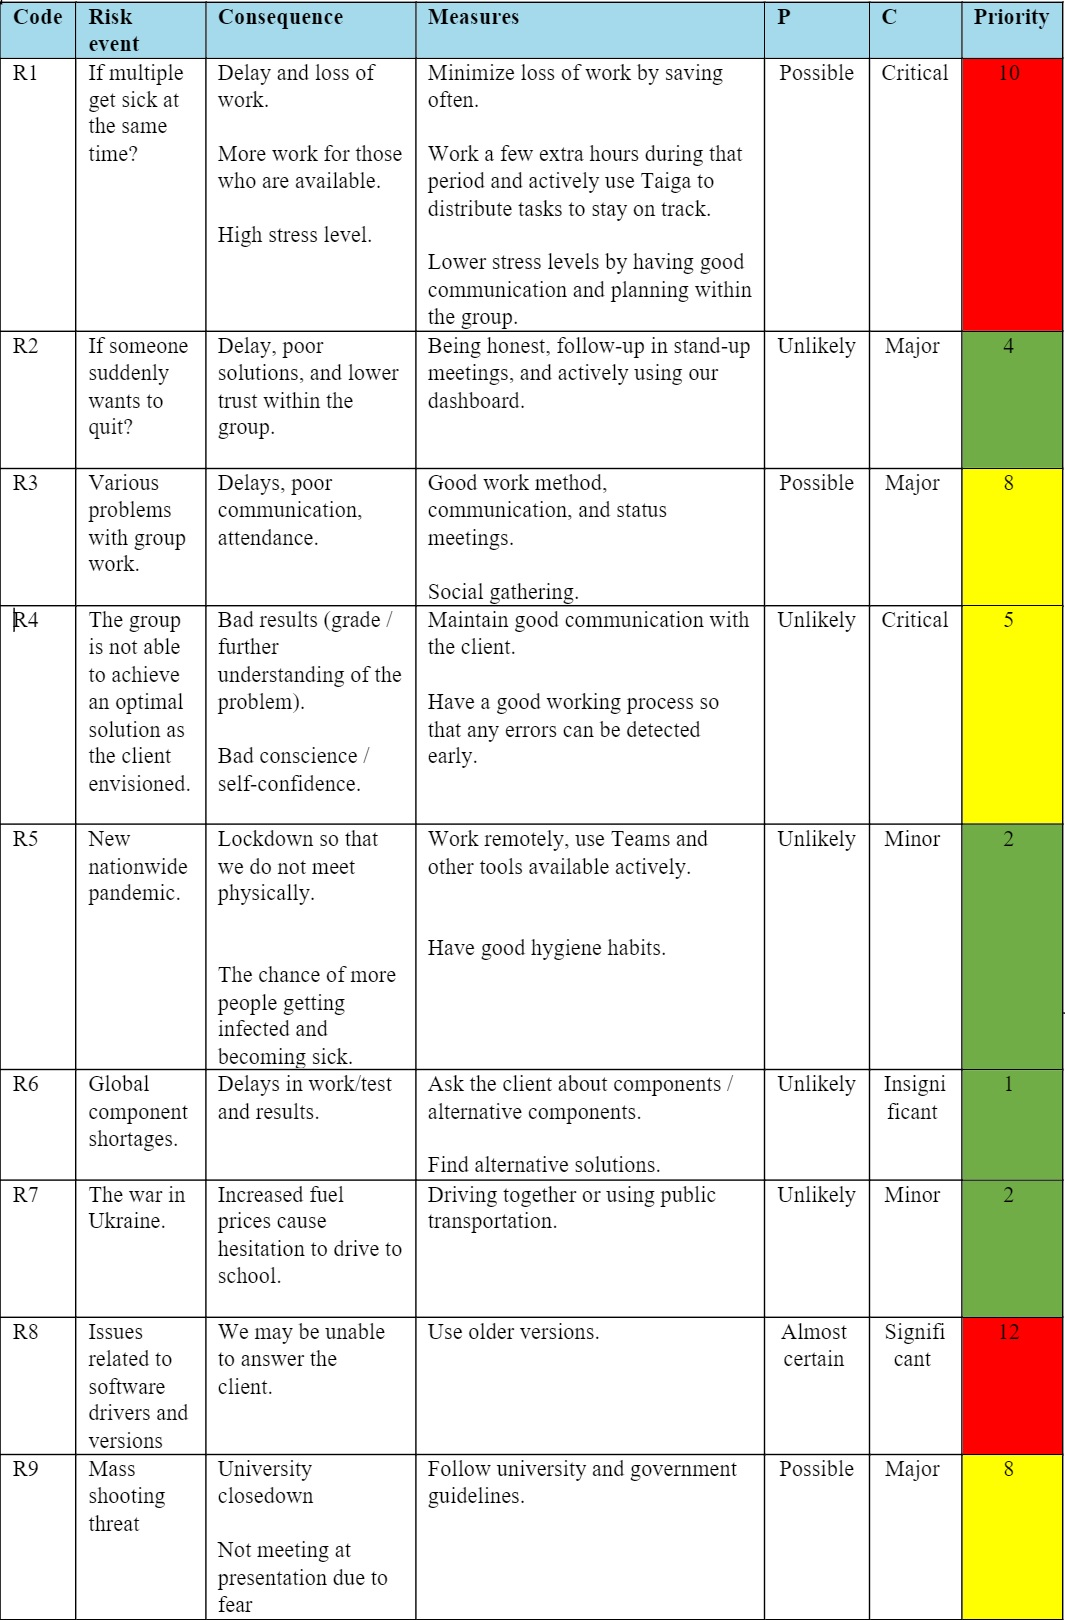
\includegraphics[width=0.80\linewidth]{fig/RisikoTabell.jpg}
\caption{Risk table}
\label{fig:Risktable}
\end{figure}

\newpage

The prioritization of these risks was determined by evaluating their consequence and probability using the risk matrix:

\begin{figure}[h!]
\centering
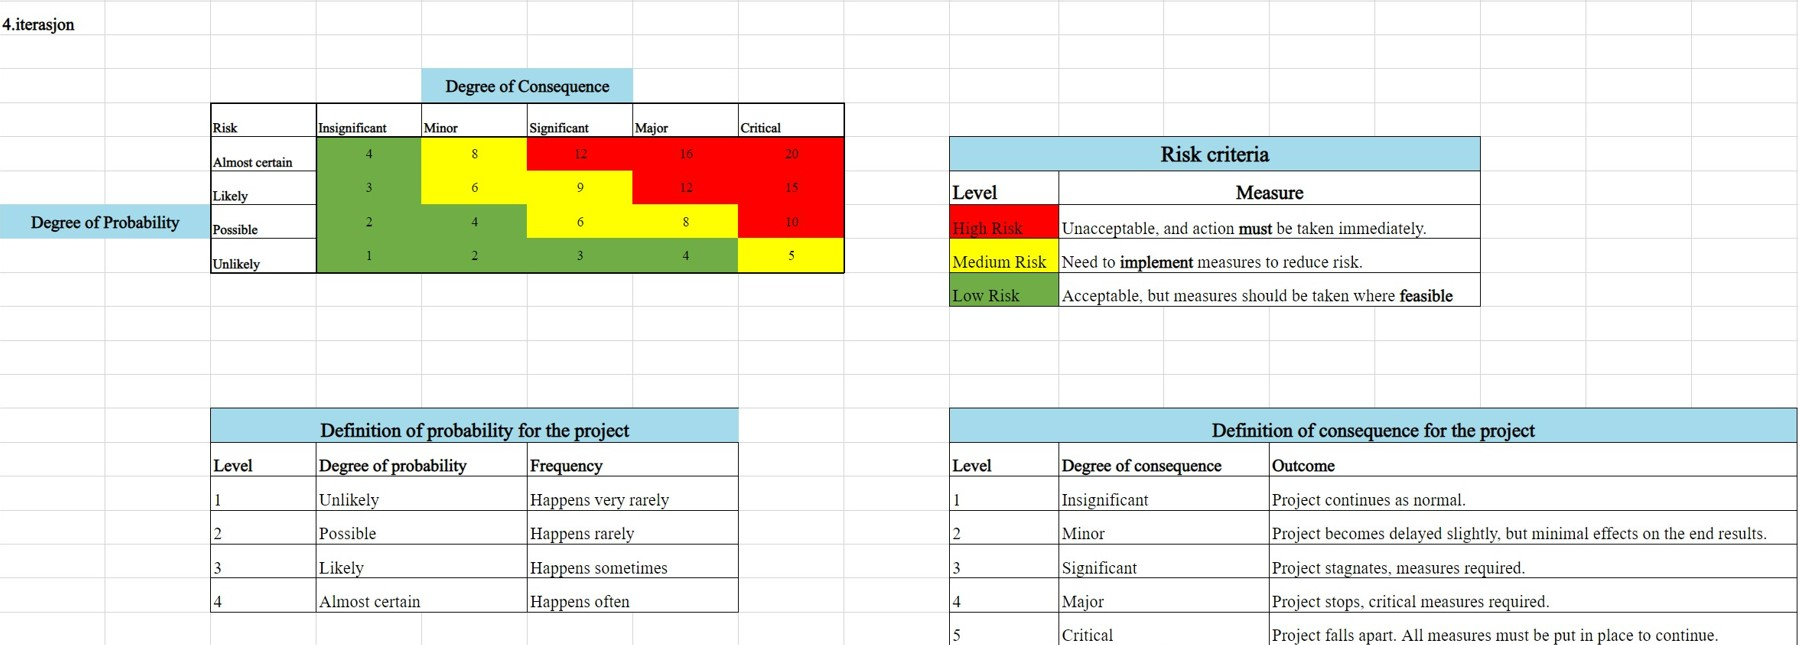
\includegraphics[width=0.85\linewidth]{fig/RiskMatrix.jpg}
\caption{Risk Matrix \cite{RiskMatrix}} 
\label{fig:RiskMatrix}
\end{figure}
\newpage